\documentclass[a4paper,french,11pt]{article}
\usepackage[top=3cm,bottom=3cm,left=3cm,right=3cm]{geometry}
\usepackage[T1]{fontenc}
\usepackage[french]{babel}
\usepackage[most]{tcolorbox}
\usepackage[utf8]{inputenc}
\usepackage{accsupp}
\usepackage{colortbl}
\usepackage{fancyhdr}
\usepackage{framed}
\usepackage{hyperref}
\usepackage{mdframed}
\usepackage{minted}
\usepackage{titlesec}
\usepackage{titling}

% Reduce minted space
\setlength\partopsep{-\topsep}
\addtolength\partopsep{-\parskip}
\addtolength\partopsep{0.3cm}

% Reduce title top margin
\setlength{\droptitle}{-5em}

\providecommand{\tightlist}{%
  \setlength{\itemsep}{0pt}\setlength{\parskip}{0pt}}

\def\pyear{2021}
% includes
\usepackage{amsmath}
\usepackage{graphicx}
\usepackage{subcaption}
\usepackage{tikz}
\usetikzlibrary{arrows.meta,decorations.pathreplacing}
% settings
\def\ptitle{Projet jeu}


\setlength{\headheight}{15pt}
\pagestyle{fancy}
\fancyhf{}
\rhead{GCC! \pyear}
\lhead{\ptitle}
\cfoot{\thepage}
\fancyfoot[L]{
\includegraphics[height=1.5\headheight]{../logo_gcc_court.pdf}}
\fancyfoot[R]{
\includegraphics[height=1.5\headheight]{../prologin_cube_bw.pdf}}

% No copy linenos : https://tex.stackexchange.com/questions/83204/how-can-i-make-source-code-included-with-minted-copyable

\newcommand\emptyaccsupp[1]{\BeginAccSupp{ActualText={}}#1\EndAccSupp{}}

\let\theHFancyVerbLine\theFancyVerbLine % don't apply our patch to hyperref's version
\def\theFancyVerbLine{\rmfamily\tiny\emptyaccsupp{\arabic{FancyVerbLine}}}

\definecolor{grey}{RGB}{240, 240, 240}
\setminted[text]{bgcolor=grey}
\setminted[python]{linenos=true,frame=single,framesep=4pt}
\setminted[html]{linenos=true,frame=single,framesep=4pt}
\setminted[css]{linenos=true,frame=single,framesep=4pt}
\setminted[js]{linenos=true,frame=single,framesep=4pt}
\newenvironment{exercise}{\begin{mdframed}[nobreak=true]}{\end{mdframed}}

\title{
    \protect\centering\protect
\includegraphics[height=3cm]{../logo_gcc_long.pdf}\\
    \vspace{.1\textheight}
    {\ptitle}
}
\author{GCC! \textendash{} Prologin}
\date{\pyear}

\begin{document}

\maketitle

% TODO rajouter une section sur l'ordre des blit et l'affichage avec update (peut-être même leur parler de surface).
% TODO détailler : les collisions, la gravité.
% TODO leur faire tester plus de truc ? Genre while True: pygame.event.get(); print(pygame.key.get_pressed()) ?

\section{Introduction}
\paragraph{}
Bravo, vous avez survécu jusqu'à la fin de la semaine !
Il est temps de passer aux choses sérieuses.
Pour clore le stage, on vous propose de coder un petit jeu qui vous fera utiliser toutes les notions que vous avez vues jusqu'ici. 
Ce sujet va vous guider à travers la réalisation d'un jeu.
Nous n'allons pas vous donner un jeu précis à programmer mais un ensemble de méthodes pour réaliser le jeu que vous aurez imaginé.

\paragraph{}
La première étape est donc d'avoir une idée approximative de ce que vous souhaitez réaliser.
N'ayant que 2 jours pour programmer ce jeu, on se limitera a des jeux en deux dimensions.
En particulier, vous choisirez un jeu avec une vue d'en haut (figure~\ref{fig:zelda}) ou un jeu avec une vue de coté (figure~\ref{fig:mario}), mais si vous avez quelque chose d'autre en tête, n'hésitez pas à en parler avec un organisateur.
Si vous ne pensez à rien, vous pouvez réimplémenter un jeu classique~: pacman, tetris, bomberman, mario, snake, morpion…

\begin{figure}[h]
	\null\hfill
	\begin{subfigure}[t]{0.4\textwidth}
		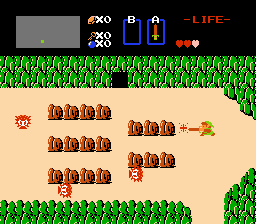
\includegraphics[width=\textwidth]{zelda.png}
		\caption{Capture d'écran de \emph{The Legend of Zelda} avec une vue d'en haut.}
		\label{fig:zelda}
	\end{subfigure}
	\hfill
	\begin{subfigure}[t]{0.4\textwidth}
		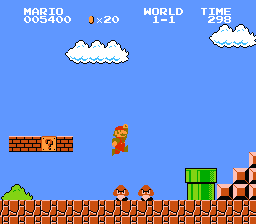
\includegraphics[width=\textwidth]{mario.png}
		\caption{Capture d'écran de \emph{Super Mario Bros.} avec une vue de coté.}
		\label{fig:mario}
	\end{subfigure}
	\hfill\null
	\caption{Comparaison des deux points de vue classiquement rencontrés dans les jeux 2D.}
	\label{fig:2dtype}
\end{figure}

\paragraph{}
Ce sujet est composé de trois parties~:
\begin{itemize}
	\item La première partie présente les bases de programmation nécessaire à la plupart des jeux, vous devez la suivre quelle que soit votre idée.
	\item La deuxième partie est une liste de fonctionnalités qui peuvent vous être utiles, par exemple il y a une section sur comment gérer le saut d'un personnage, mais celle-ci ne devrait vous être utile que si vous contrôlez un personnage en vue de coté.
	\item La troisième partie est une référence listant des fonctions disponibles dans la bibliothèque logicielle Pygame que vous allez utiliser pour implémenter votre jeu.
\end{itemize}

\paragraph{}
Si vous regardez attentivement les captures d'écran de la figure~\ref{fig:2dtype}, vous remarquerez que des images sont répétées, par exemple le sol de la figure~\ref{fig:mario} est composé d'une même image répétée une quinzaine de fois horizontalement.
Ces images de base sont appelées \emph{sprites}, ce sont les briques de bases permettant de construire un jeu visuellement riche.
Dans un premier temps, on vous demandera de vous limiter aux \emph{sprites} que nous vous avons fournies et qui sont listées en annexe~\ref{sec:sprites}.
% Lorsque vous choisissez vos sprites (images pour le jeu), essayez de sélectionner des sprites de même taille (par exemple, \(32\times32\) pixels).

\paragraph{}
Le programme que vous allez écrire va être long et il est important que vous soyez toujours capables de le comprendre demain.
Par ailleurs, la gentillesse des organisateurs est proportionnelle à la lisibilité de votre code.
C'est pourquoi, il vous est fortement conseillé de bien formater votre code et d'écrire pleins de petites fonctions chacune se chargeant d'une partie de la logique du jeu, par exemple on pourra avoir une fonction \texttt{afficher\_carte} et une autre \texttt{gerer\_deplacements}.
En écrivant de grosses fonctions monstrueuses vous nuisez à la santé des gentils organisateurs.
% N’hésitez pas à utiliser l’interpréteur python pour tester toutes les fonctions qu’on vous présente et voir comment elles se comportent. 

\section{Fondamentaux}

\paragraph{}
Pour commencer, nous allons vous guider à travers l'affichage des \texttt{sprites} et comment les faire se déplacer.
Pour programmer votre jeu, vous allez utiliser la bibliothèque Pygame, toutes les fonctions de cette bibliothèque commenceront donc par \texttt{pygame.}, par exemple \texttt{pygame.transform.scale}.

\subsection{Structure du programme}
\label{sec:structure}

\paragraph{}
On distinguera deux partie à votre programme~: l'initialisation et la boucle de jeu.
L'initialisation n'est faite qu'une seule fois au début du programme, alors que la boucle de jeu va être exécutée une centaine de fois par seconde.
Par exemple, dans la partie initialisation on initialisera le score du joueur à 0~: \mintinline{python}{score = 0}, alors que dans la boucle de jeu on augmentera le score du joueur lorsque certaines conditions sont vérifiées \mintinline{python}{score += 1}.
Tout au long du projet, il vous faudra faire bien attention à ne pas écrire du code trop lent dans la boucle de jeu, si vous voulez que la boucle s'exécute 100 fois par seconde, il est nécessaire qu'une itération prenne moins de 10 millisecondes.

\paragraph{}
La bibliothèque Pygame nécessite d'être initialisée, pour cela vous utiliserez la fonction \texttt{pygame.init}, vous commencerez votre programme par~:
\begin{minted}{python}
import pygame

# Initialisation
pygame.init()

while True:
    # Boucle de jeu
\end{minted}

\subsection{L'écran}
\label{sec:ecran}

\paragraph{}
Pour la plupart des programmes, l'unité d'affichage de base est le pixel~: un carré de l'ordre d'un dixième de millimètre de coté qui ne peut être que d'une seule couleur donnée.
L'écran peut être vu comme une grille de pixels, la particularité étant que l'origine se trouve en haut à gauche (voir figure~\ref{fig:ecran}).

\paragraph{}
La première étape que vous allez tester est l'ouverture d'une fenêtre.
Pour ce faire vous utiliserez la fonction \texttt{pygame.display.set\_mode} qui prend en argument une paire d'entiers~: \((\text{largeur}, \text{hauteur})\), la taille de la nouvelle fenêtre.
Cette fonction renvoie un objet représentant la fenêtre ainsi créée, il sera nécessaire de passer cet objet à d'autres fonctions pour pouvoir dessiner dedans, gardez le dans une variable~!
Il n'est nécessaire de créer qu'une seule fenêtre au début du programme, cet appel de fonction va donc dans la partie initialisation.

\begin{figure}[t]
\begin{tikzpicture}
	\draw (0,0) rectangle (9.6, 5.4);
	\draw[-{Latex},red] (-0.2,5.4) -- (-0.2, 0);
	\draw[-{Latex},red] (0,5.6) -- (9.6, 5.6);

	\node at (-0.5,5.7) {\((0, 0)\)};
	\node at (-0.5,-0.3) {\((0, 1080)\)};
	\node at (9.5,-0.3) {\((1920, 1080)\)};
	\node at (9.5,5.9) {\((1920, 0)\)};

	\node at (4.4,3.6) {\((700, 300)\)};

	\draw[blue] (0,3.9) -- (3.5,3.9);
	\draw[blue] (3.5,5.4) -- (3.5,3.9);
	\draw[decorate,decoration={brace,amplitude=5,mirror},xshift=0,yshift=0] (0,3.9) -- (3.5,3.9) node[black,midway] (sx) {};
	\draw[decorate,decoration={brace,amplitude=5},xshift=0,yshift=0] (3.5,5.4) -- (3.5,3.9) node[black,midway] (sy) {};
	\filldraw[blue] (3.5, 3.9) circle (0.075);

	\node at (1.75,3.55) {700};
	\node at (4.05,4.65) {300};
\end{tikzpicture}
	\caption{Illustration du système de coordonnées d'un écran de 1920 pixels de largeur et 1080 pixels de hauteur. Le point \((700, 300)\) est marqué en bleu.}
	\label{fig:ecran}
\end{figure}

\paragraph{}
La seconde fonction dont vous aurez besoin est \texttt{pygame.display.update}.
Cette fonction (qui ne prend pas d'argument) va dessiner le contenu de la fenêtre à l'écran.
Cette action doit être effectuée à chaque tour de boucle, votre programme va donc demander à la bibliothèque Pygame de dessiner l'écran plus d'une centaine de fois par seconde~!

\paragraph{}
Votre programme devrait donc ressembler au code suivant~:
\begin{minted}{python}
import pygame

# Initialisations
pygame.init()
ecran = pygame.display.set_mode((800, 600))
# …

while True:
    # Boucle de jeu
    # …
    pygame.display.update()
\end{minted}
Écrivez et exécutez ce code.
Pour l'instant on n'affiche rien, la fenêtre reste donc vide.

\paragraph{}
Une première fonction que vous pouvez ajouter est~:
\begin{minted}{python}
ecran.fill(pygame.Color('blue'))
\end{minted}
Celle-ci se place dans la boucle de jeu et vous permet de changer la couleur de fond de la fenêtre.
Pour choisir la couleur, vous pouvez écrire le nom de la couleur en anglais, une valeur hexadécimale comme en HTML (\texttt{"\#8000FF"}) ou des valeurs RGB entre 0 et 255.

\subsection{Rectangles}
\label{sec:rectangles}

\paragraph{}
La bibliothèque Pygame fait un usage intensif d'objets de type Rectangle.
Pour créer un nouveau rectangle vous pouvez utiliser \texttt{pygame.Rect} qui prend 4 arguments \((x, y, w, h)\) où \((x,y)\) sont les coordonnées du coin supérieur gauche du rectangle et \(w\) et \(h\) sont respectivement la largeur (\emph{width}) et la hauteur (\emph{height}) du rectangle.
Par exemple, sur la figure~\ref{fig:ecran}, le rectangle en haut à gauche délimité par les traits bleus correspond au rectangle \texttt{pygame.Rect(0, 0, 700, 300)}.

\paragraph{}
De nombreux descripteurs sont disponibles pour accéder aux différents points d'intérêt d'un rectangle, lorsque vous avez défini une variable \texttt{r} comme étant un rectangle, vous pouvez accéder au point supérieur gauche avec \texttt{r.x} et \texttt{r.y}, à sa taille avec \texttt{r.w} et \texttt{r.h}, mais aussi aux coordonnées de son centre avec \texttt{r.centerx} et \texttt{r.centery}, ou encore à son coté droit avec \texttt{r.right}, son coté inférieur avec \texttt{r.bottom}, etc…

\paragraph{}
Pour dessiner un rectangle coloré, Pygame met à votre disposition la fonction \texttt{pygame.draw.rect} dans la boucle de jeu, par exemple~:
\begin{minted}{python}
rectangle = pygame.Rect(100, 300, 200, 100)
pygame.draw.rect(ecran, pygame.Color('red'), rectangle)
\end{minted}

\paragraph{}
Les rectangles sont des objets dit \emph{mutables}, cela signifie que lorsque \texttt{r1} est un rectangle et que vous écrivez \texttt{r2 = r1}, cela ne crée pas de nouveau rectangle mais donne juste un nouveau nom au rectangle \texttt{r1} déjà existant.
En particulier, faites bien attention au code suivant~:
\begin{minted}{python}
import pygame
r1 = pygame.Rect(2, 2, 10, 10)
r2 = r1
r1.x = 3
print(r2.x)
\end{minted}
Celui-ci affiche 3 et non 2 comme on pourrait s'y attendre\footnote{Si \texttt{r1} et \texttt{r2} étaient des entiers ce code afficherait bien 2.}.
Pour effectuer une vraie copie du rectangle \texttt{r1}, il faudra remplacer la ligne~4 par \texttt{r2 = r1.copy()}.

\subsection{Images}
\label{sec:images}

\paragraph{}
Nous allons finalement passer à l'affichage d'images, cela se fait en deux parties~: d'abord l'image est chargée en mémoire, puis elle est affichée dans une fenêtre à proprement parler.
Pour charger une image, vous utiliserez l'appel suivant~:
\begin{minted}{python}
image = pygame.image.load("chemin/sprite.png").convert_alpha()
\end{minted}
La fonction \texttt{pygame.image.load} prend en argument le chemin vers un fichier image et charge ce fichier en mémoire.
La fonction \texttt{convert\_alpha} permet quant à elle de convertir l'image dans un format rapide et optimisé pour Pygame.
Ces deux fonctions sont plutôt lentes, il faut donc les appeler dans la partie initialisation, ne chargez pas d'image dans la boucle de jeu, c'est bien trop lent~!

\paragraph{}
Une fonction utile sur les images est \texttt{get\_rect}, celle-ci permet de récupérer un rectangle de la taille de l'image.
Le rectangle ainsi retourné est ancré en \((0, 0)\) et est de la même taille que l'image.

\paragraph{}
Enfin, pour afficher l'image, il faut utiliser la fonction \texttt{blit} sur l'objet \texttt{ecran} renvoyé par la fonction \texttt{pygame.display.set\_mode} vu à la section~\ref{sec:ecran}.
Cette fonction prend deux arguments~: l'image à afficher (que vous avez chargée avec la fonction \texttt{pygame.image.load}) et un rectangle où afficher cette image.
Il faudra que ce rectangle soit de la même taille que l'image a afficher.
En général, on utilise la fonction \texttt{get\_rect} pour cela, on a alors un code de la forme~:
\begin{minted}{python}
rectangle = image.get_rect()
rectangle.x = 200
rectangle.y = 100
ecran.blit(image, rectangle)
\end{minted}
Ce code qui affiche une image aux coordonnées \((200, 100)\), doit être écrit dans la boucle de jeu.
Essayez d'afficher une image, si vous avez un soucis, appelez un organisateur.

\paragraph{}
Remarquez que changer la taille du rectangle (par exemple \texttt{rectangle.w}), ne suffit pas pour changer la taille de l'image.
Pour ce faire, il faudra d'abord redimensionner l'image comme vu section~\ref{sec:transform}.

\subsection{Évènements}
\label{sec:evenements}

\paragraph{}
Pour communiquer avec le programme, l'utilisateur (dans ce cas là, le joueur) va envoyer des \emph{évènements} au programme.
Un événement peut prendre de nombreuses formes~: c'est l'appui sur une touche du clavier ou un mouvement de la souris, mais également la fermeture d'une fenêtre, sa réduction ou son redimensionnement.
Pour faire court, toute interaction avec le programme se fait à travers des évènements.

\paragraph{}
Le premier événement que vous allez capturer est la fermeture du programme.
Pour fermer la fenêtre Pygame, il faut utiliser l'appel de fonction \texttt{pygame.quit()} qui est un peu l'inverse de \texttt{pygame.init()}.
Puis, pour arrêter votre programme à proprement parler, nous allons utiliser l'appel de fonction \texttt{sys.exit(0)}, pour cela il est nécessaire d'ajouter \texttt{import sys} lors de l'initialisation du programme.
Cet appel permet de sortir directement du programme sans avoir à attendre que toutes les instructions soient exécutées.
\begin{minted}{python}
for evenement in pygame.event.get():
    if evenement.type == pygame.QUIT:
        pygame.quit()
        sys.exit(0)
\end{minted}

\paragraph{}
Le traitement des évènements doit impérativement se faire dans la boucle de jeu~: on va vérifier une centaine de fois par seconde si l'utilisateur a appuyé sur une touche ou, dans ce cas là, s'il a fermé le programme.
La fonction \texttt{pygame.event.get} renvoie une liste des événements ayant eu lieu depuis le dernier tour de boucle.
Si vous êtes curieux du type d'évènement reçu par le programme vous pouvez ajouter une ligne \texttt{print(evenement)} avant le \texttt{if} et regarder ce qui est affiché quand vous bougez la souris ou utilisez le clavier dans la fenêtre du jeu.
Pour chaque évènement reçu, on vérifie si son type est \texttt{pygame.QUIT}, si un tel évènement a eu lieu, on ferme le programme.

\subsection{Déplacements}
\label{sec:deplacements}

\paragraph{}
Avant de regarder comment capturer les évènements correspondants à l'appui d'une touche du clavier, nous allons voir comment déplacer des images.
Cela se fait très simplement~: il suffit de redessiner la même image à des emplacements différents.
Par exemple, initialisez une variable \texttt{posx} à 0 hors de la boucle de jeu, puis incrémentez là à chaque tour de boucle pour compter combien de tours ont été effectués jusqu'à présent.
Vous pouvez maintenant modifier la position du rectangle où vous dessinez votre image pour que celle-ci dépende de \texttt{posx}.
Par exemple, au lieu de faire \texttt{rectangle.x = 100}, vous pouvez faire \texttt{rectangle.x = posx}.

\paragraph{}
Essayez d'afficher une image qui se déplace en diagonale, du coin supérieur gauche vers le coin inférieur droit.

\subsection{Utiliser le clavier}
\label{sec:clavier}

\paragraph{}
La capture des touches du clavier peut se faire comme vu à la section~\ref{sec:evenements}, à l'aide de la fonction \texttt{pygame.event.get} tout comme \texttt{pygame.QUIT}, mais pour chaque touche du clavier, Pygame a deux évènements~: un lorsque la touche est enfoncée et un autre lorsque la touche est relachée.
Traiter les évènements de cette manière est très fastidieux, pour nous simplifier la tâche, une autre fonction est disponible~: \texttt{pygame.key.get\_pressed}.
Cette fonction renvoie un tableau avec autant de valeur que de touche sur le clavier, initialement toutes les valeurs sont 0.
Lorsqu'une touche est enfoncée la case du tableau correspondante est mise à 1.
Pour savoir si la touche droite est enfoncée on pourra regarder la valeur du tableau en l'indice \texttt{pygame.K\_RIGHT}~:
\begin{minted}{python}
touches = pygame.key.get_pressed()
if touches[pygame.K_RIGHT] == 1:
    print("Touche droite enfoncée")
\end{minted}
De même que \texttt{pygame.K\_RIGHT} désigne la flèche de droite, il existe une variable Pygame pour chaque touche du clavier, celles-ci sont listées section~\ref{sec:refclavier}.

\paragraph{}
Si vous recopiez le code ci-dessus, une ligne sera écrite dans le terminal à chaque tour de boucle lorsque la flèche droite est enfoncée.
En vous inspirant de la section~\ref{sec:deplacements}, modifiez votre programme pour pouvoir déplacer une image à gauche et à droite à l'aide des flèches directionnelles.

\subsection{Carte d'un niveau}
\label{sec:carte}

\paragraph{}
Écrire autant de \texttt{blit} que d'image à l'écran est beaucoup trop long et fastidieux.
On préfèrera utiliser un tableau représentant la carte du jeu.
Pour cela, chargez deux images~: \texttt{image1} et \texttt{image2} et créez un tableau comme suit~:
\begin{minted}{python}
carte = [[1, 1, 1, 1],
         [1, 0, 0, 1],
         [1, 0, 2, 1],
         [1, 1, 1, 1]]
\end{minted}
Vous pouvez alors itérer sur le tableau \texttt{carte} avec deux boucles \texttt{for} imbriquées.
Lorsque vous rencontrez un 1, faites \texttt{blit} d'\texttt{image1}, lorsque vous rencontrez un 2, faites un \texttt{blit} d'\texttt{image2} et lorsque vous rencontrez un 0, ne faites rien.
Toute la difficulté réside en savoir où \texttt{blit} ces images.
En effet la fonction \texttt{blit} prend le rectangle où dessiner l'image en paramètre.
Il faudra donc faire dépendre les coordonnées de ce rectangle des indices des deux boucles \texttt{for}.
Le résultat que vous devriez obtenir est donné figure~\ref{fig:carte}.

\begin{figure}[t]
	\centering
	
\includegraphics[width=.5\textwidth]{carte.png}
	\caption{Rendu du tableau \texttt{carte} dans une fenêtre de taille \(800\times 600\) en utilisant les \emph{sprites} \texttt{grassCenter.png} pour \texttt{image1} et \texttt{snowCenter.png} pour \texttt{image2}.}
	\label{fig:carte}
\end{figure}

\subsection{Gestion des collisions}
\label{sec:collisions}

\paragraph{}
Enfin, si vous avez implémenté les sections~\ref{sec:clavier} et \ref{sec:carte}, vous avez dû remarquer qu'il est possible d'utiliser les touches directionnelles pour déplacer l'image n'importe où, y compris hors de la carte.
Pour empêcher les mouvements hors de la carte, vous pouvez commencer par limiter la position de l'image lorsque celle-ci est déplacée~: si une coordonnée passe en dessous de zéro, celle-ci est laissée à zéro à la place.

\paragraph{}
La collision avec d'autres images est plus difficile à gérer.
Il est nécessaire de commencer par stocker une liste des rectangles solides qui ne pourront pas être traversés.
Un bon endroit pour faire cela est dans la boucle de dessin de la carte~: on commence avec une liste vide \texttt{solides = []}, puis pour chaque \texttt{i}, \texttt{j}, si \texttt{carte[i][j]} représente un objet solide, le rectangle correspondant est ajouté à \texttt{solides}.

\paragraph{}
Lorsqu'une touche est pressée, on va mettre à jour les coordonnées d'une image à condition que le nouveau rectangle n'a pas d'intersection avec un rectangle de la liste \texttt{solides}.
Pour tester s'il existe une intersection entre deux rectangles \texttt{r1} et \texttt{r2}, Pygame nous fournit la fonction~:
\begin{minted}{python}
collision = r1.colliderect(r2)
if collision:
    # ne pas se déplacer…
\end{minted}
Où \texttt{collision} est un booléen égal à \texttt{True} s'il existe une collision, \texttt{False} sinon.

\paragraph{}
Avec la technique décrite ci-dessus vous remarquerez que l'image ne s'approche pas totalement des murs comme on s'y attendrait.
Pour pallier à cela, une fois que vous avez trouvé le rectangle solide avec lequel vous êtes en collision, vous pouvez effectuer un mouvement de la forme~:
\begin{minted}{python}
personnage.left = solide.right
\end{minted}
Cette ligne permet de déplacer la gauche du personnage de telle manière à ce que ce soit exactement la droite du solide.
Cette action est donc à effectuer si on trouve une collision à gauche, c'est à dire lorsque l'on se déplace vers la gauche et qu'on rencontre un obstacle.
Une code similaire devra être écrit pour toutes les directions (\texttt{left}, \texttt{right}, \texttt{top}, \texttt{bottom}).

\paragraph{}
Finalement, pour gérer correctement les mouvements diagonaux, il vous est fortement conseillé de séparer votre détection de collision en deux parties~:
\begin{itemize}
	\item Essayer de se déplacer horizontalement
	\item Résoudre les collisions horizontales
	\item Essayer de se déplacer verticalement
	\item Résoudre les collisions verticales
\end{itemize}
Cet ordre d'action vous assure que vos images ne se bloqueront pas dans les coins des solides de la carte.

\section{Pour aller plus loin}

\paragraph{}
Cette section présente plusieurs fonctionnalités qui ne vous seront pas nécessairement utiles, vous pouvez directement regarder les parties qui vous intéressent.

\subsection{Écrire du texte}
\label{sec:texte}

\paragraph{}
Pour écrire un texte à l'écran, il faut commencer par choisir la police d'écriture à l'aide de la fonction \texttt{pygame.font.Font}, cette fonction prend deux arguments~: le nom de la police d'écriture et sa taille.
Il est aussi possible de remplacer le nom de la police par \texttt{None} pour laisser la police par défaut.

À partir d'une police d'écriture, il nous est possible de générer du texte avec \texttt{police.render} qui prend trois arguments~: le texte à afficher, antialiasing\footnote{Qu'on laissera toujours à \texttt{True}.} et la couleur du texte.
Après cela, afficher du texte se fait comme afficher une image, avec \texttt{ecran.blit}.
On obtient alors un code de la forme~:
\begin{minted}{python}
police = pygame.font.Font(None, 50)
texte = police.render("Mon texte", True, pygame.Color('green'))
rectangle = texte.get_rect()
ecran.blit(texte, rectangle)
\end{minted}

\subsection{Utiliser la souris}
\label{sec:souris}

\paragraph{}
Les clics de souris peuvent être extrêmement rapides, on préféra les récupérer dans la boucle d'évènements en même temps que \texttt{pygame.QUIT}.
Il faudra donc voir si l'un des évènements est l'appui sur le clic gauche~:
\begin{minted}{python}
if evenement.type == pygame.MOUSEBUTTONDOWN:
    # …
\end{minted}

Il est alors possible de récupérer la position de la souris avec la fonction \texttt{pygame.mouse.get\_pos} qui renvoie une paire d'entiers \((x, y)\), la position relative au pixel en haut à gauche~:
\begin{minted}{python}
if evenement.type == pygame.MOUSEBUTTONDOWN:
    position = pygame.mouse.get_pos()
    souris_x = position[0]
    souris_y = position[1]
    print(souris_x, souris_y)
\end{minted}

\subsection{Évènements aléatoires~: le module \texttt{random}}
\label{sec:random}

\paragraph{}
Pour introduire des éléments aléatoires dans votre jeu, il vous est possible d'utiliser le module python \texttt{random}.
Après avoir importé le module avec \texttt{import random} dans la partie initialisation, vous pouvez faire appel aux fonctions suivantes~:
\begin{itemize}
	\item \texttt{random.randint(a, b)} renvoie un nombre entier uniformément distribué entre \texttt{a} et \texttt{b} inclus.
	\item \texttt{random.random()} renvoie un nombre à virgule uniformément distribué entre 0 inclus et 1 exclu.
\end{itemize}

La fonction \texttt{random.randint} peut par exemple être utilisée pour simuler le lancer d'un dé à 6 faces~:
\begin{minted}{python}
de1 = random.randint(1, 6)
de2 = random.randint(1, 6)
if de1 == 6 and de2 == 6:
    print("Double 6 !")
\end{minted}

\subsection{Gestion du temps~: le module \texttt{time}}
\label{sec:time}

\paragraph{}
Vous pouvez stocker dans une variable l'état actuel de l'horloge grâce à la fonction \texttt{time.time}.
Vous pouvez ensuite soustraire cette variable à un second appel pour connaître le nombre de secondes écoulées.
Par exemple, dans la partie initialisation vous pouvez ajouter~:
\begin{minted}{python}
import time
debut = time.time()
\end{minted}
Puis lors de la gestion des appuis sur les touches du clavier (voir la section~\ref{sec:clavier})~:
\begin{minted}{python}
if touches[pygame.K_SPACE] == 1:
    print(time.time() - debut, "secondes")
\end{minted}
Avec ces deux lignes, appuyer sur espace affiche le nombre de secondes écoulées depuis le lancement du jeu.

\subsection{Fluidité du jeu~: fixer la durée d'une boucle}
\label{sec:fps}

\paragraph{}
Dans la boucle de jeu, il est parfois nécessaire d'effectuer des opérations complexes qui ralentissent le programme.
Par conséquent, le jeu peut paraitre moins fluide, les personnages se déplaçant en saccade.
Pour contrer cela, il est possible de donner une durée minimale à un tour de boucle avec un objet horloge de Pygame.
Dans la partie initialisation, vous pouvez ajouter la ligne~:
\begin{minted}{python}
horloge = pygame.time.Clock()
\end{minted}
Puis à la fin de la boucle de jeu vous pouvez faire~:
\begin{minted}{python}
horloge.tick(60)
\end{minted}
Où 60 est le nombre de tour de boucle qui seront effectués chaque seconde.
Ce nombre doit généralement être plus grand que 30 pour obtenir un jeu un minimum fluide.
C'est ce que l'on appelle couramment les \emph{FPS} (\emph{frames per second}, images par seconde).
En pratique, la fonction \texttt{horloge.tick} va volontairement stopper le programme quelques millisecondes lorsque la boucle tourne trop vite.
Après \texttt{horloge.tick}, vous pouvez ajouter un \texttt{print(horloge.get\_fps())} pour vérifier que vous avez bien 60 tours de boucle par seconde.

\subsection{Saut réaliste~: vitesse et gravité}
\label{sec:gravite}

\paragraph{}
Lorsque vous avez un personnage, sa position sur l'écran peut être vue comme un vecteur \(\vec{p}\) en deux dimensions \(\vec{p} = (p_x, p_y)\).
C'est les deux premières valeurs du rectangle correspondant à la sprites du personnage.
On peut également considérer un vecteur \(\vec{v}\) qui représente la vitesse de déplacement du personnage.
À chaque tour de boucle \(v_x\) et \(v_y\) sont mis à zéro et si le joueur appuie sur la flèche gauche, \(v_x\) est mis à \(-3\) pour que le personnage se déplace de 3 pixels par tour de boucle.
Une fois la vitesse calculée, on change le vecteur \(\vec{p}\) en \(\vec{p}+\vec{v}\) pour déplacer le personnage\footnote{N'oubliez pas de faire ça en deux fois~: d'abord le déplacement horizontalement (\(p_x\) est transformé en \(p_x + v_x\)), suivi de la résolution des collisions (voir section~\ref{sec:collisions}), puis déplacement vertical, suivi d'une autre phase de résolution des collisions.}.

\paragraph{}
Pour avoir un saut réaliste, il ne faut pas remettre \(v_y\) à 0 à chaque tour de boucle.
Plutôt, il faut l'incrémenter à chaque tour de boucle \(v_y \gets v_y + 1\), cela correspond à l'effet de la gravité qui nous pousse en permanence vers le bas.
Par ailleurs, lorsque la touche de saut est appuyée, il suffit de donner une impulsion vers le haut au personnage en fixant \(v_y \gets -20\).
Le saut prendra donc la forme suivante~:
\begin{itemize}
	\item Au premier tour de boucle \(v_y\) est -20, le personnage se déplace vers le haut de 20 pixels.
	\item Au second tour de boucle \(v_y\) est affecté par la gravité et passe à -19, le personnage se déplace vers le haut de 19 pixels.
	\item …
	\item Au vingt-et-unième tour de boucle, la gravité passe \(v_y\) de -1 à 0, le personnage ne bouge plus.
	\item Au vingt-deuxième tour de boucle, la gravité passe \(v_y\) de 0 à 1, le personnage commence à retomber de 1 pixel.
	\item Au vingt-troisième tour de boucle, la gravité passe \(v_y\) de 1 à 2, le personnage tombe de 2 pixels.
	\item Au vingt-quatrième tour de boucle, la gravité passe \(v_y\) de 2 à 3, le personnage tombe de 3 pixels.
	\item …
\end{itemize}
Vous remarquerez que quand le personnage retombe, il gagne de la vitesse à chaque tour de boucle, comme on peut l'observer dans la vie réelle.
En pratique le saut va former une parabole, c'est la trajectoire standard d'un objet affecté par la gravité.

\paragraph{}
Pour gérer ça dans votre code, en plus de stocker la position du personnage comme vous devez déjà le faire, stockez également deux valeurs~: la vitesse horizontale et la vitesse verticale.
Dans la gestion des évènements, au lieu d'ajouter une valeur directement à la position du personnage, changez la vitesse.
Si vous rencontrez une collision en dessous du personnage, n'oubliez pas de mettre la vitesse verticale à 0, cela correspond à toucher le sol.

\subsection{Mouvements réalistes~: Animation des \emph{sprites}}
\label{sec:animation}

\paragraph{}
Pour animer un personnage, rien de plus simple~: il suffit d'afficher une image différente à chaque tour de boucle du jeu.
Regardez les images disponibles en annexe~\ref{sec:spritesanimes}, il y a par exemple 2 images pour un personnage immobile (les images \emph{standing}).
Pour les utiliser, il faut commencer par stocker dans une variable le tour de boucle actuel~: initialisez une variable \texttt{tour\_de\_boucle} à 0, puis à chaque tour de boucle incrémentez là de 1.
Si vous changiez l'image exactement à chaque tour de boucle, l'animation risque d'être beaucoup trop rapide, du coup on préfèrera choisir l'image en fonction de \texttt{tour\_de\_boucle // 50 \% 2}, cette valeur sera 0 pour les 50 premiers tours de boucle, puis 1 pour les 50 suivants, puis de nouveau 0 pour les 50 suivants, etc.
Du coup, au lieu \texttt{blit} toujours la même image du personnage, alternez entre les deux images disponibles selon la valeur de \texttt{tour\_de\_boucle // 50 \% 2}.

\paragraph{}
Pour simplifier l'écriture du code, il est bien plus facile de mettre les images dans un tableau, vous pouvez même utiliser une compréhension de liste (la syntaxe avec un \texttt{for} entre des crochets) pour charger toutes les images à la fois\footnote{Ici le \texttt{\%d} sera remplacé par \texttt{i} à chaque tour de boucle, c'est une syntaxe particulière pour inclure un nombre dans une chaine de caractères.}~:
\begin{minted}{python}
court = [pygame.image.load(
        "sprites/anime/p1/running/frame-%d.png" % i
    ).convert_alpha()
    for i in range(1,7)]
\end{minted}

\paragraph{}
Pour choisir quelle image afficher, il suffit de regarder la vitesse du personnage (voir section~\ref{sec:gravite}).
Par ailleurs, il vous est possible de stocker une variable direction pour savoir dans quelle direction le personnage est orienté.
Grâce à la fonction \texttt{pygame.transform.flip} (voir section~\ref{sec:transform}), il vous est alors possible d'afficher un personnage regardant vers la gauche.

\section{Référence}
\label{sec:reference}

\subsection{Touches du clavier}
\label{sec:refclavier}
Les lettres sont facilement accessible, par exemple la touche x est désignée par \texttt{pygame.K\_x}.
Il en va de même pour les chiffres et les touches F1 à F12.
Pour les autres touches il faut connaitre les traductions anglaises, dans le doute demandez à un organisateur.
Les touches directionnelles sont \texttt{pygame.K\_left}, \texttt{pygame.K\_right}, \texttt{pygame.K\_up}, \texttt{pygame.K\_down}.
Les touches espaces et entrée sont respectivement \texttt{pygame.K\_SPACE} et \texttt{pygame.K\_RETURN}.
Hormis cela, les autres touches disponibles sont~:
\begin{center}
\begin{tabular}{l l l l}
\texttt{K\_AMPERSAND} & \texttt{K\_GREATER}      & \texttt{K\_KP\_PERIOD}  & \texttt{K\_POWER}        \\
\texttt{K\_ASTERISK}  & \texttt{K\_HASH}         & \texttt{K\_KP\_PLUS}    & \texttt{K\_PRINT}        \\
\texttt{K\_AT}        & \texttt{K\_HELP}         & \texttt{K\_LALT}        & \texttt{K\_QUESTION}     \\
\texttt{K\_BACKQUOTE} & \texttt{K\_HOME}         & \texttt{K\_LAST}        & \texttt{K\_QUOTE}        \\
\texttt{K\_BACKSLASH} & \texttt{K\_INSERT}       & \texttt{K\_LCTRL}       & \texttt{K\_QUOTEDBL}     \\
\texttt{K\_BACKSPACE} & \texttt{K\_KP0}          & \texttt{K\_LEFTBRACKET} & \texttt{K\_RALT}         \\
\texttt{K\_BREAK}     & \texttt{K\_KP1}          & \texttt{K\_LEFTPAREN}   & \texttt{K\_RCTRL}        \\
\texttt{K\_CAPSLOCK}  & \texttt{K\_KP2}          & \texttt{K\_LESS}        & \texttt{K\_RIGHTBRACKET} \\
\texttt{K\_CARET}     & \texttt{K\_KP3}          & \texttt{K\_LMETA}       & \texttt{K\_RIGHTPAREN}   \\
\texttt{K\_CLEAR}     & \texttt{K\_KP4}          & \texttt{K\_LSHIFT}      & \texttt{K\_RMETA}        \\
\texttt{K\_COLON}     & \texttt{K\_KP5}          & \texttt{K\_LSUPER}      & \texttt{K\_RSHIFT}       \\
\texttt{K\_COMMA}     & \texttt{K\_KP6}          & \texttt{K\_MENU}        & \texttt{K\_RSUPER}       \\
\texttt{K\_DELETE}    & \texttt{K\_KP7}          & \texttt{K\_MINUS}       & \texttt{K\_SCROLLOCK}    \\
\texttt{K\_DOLLAR}    & \texttt{K\_KP8}          & \texttt{K\_MODE}        & \texttt{K\_SEMICOLON}    \\
\texttt{K\_END}       & \texttt{K\_KP9}          & \texttt{K\_NUMLOCK}     & \texttt{K\_SLASH}        \\
\texttt{K\_EQUALS}    & \texttt{K\_KP\_DIVIDE}   & \texttt{K\_PAGEDOWN}    & \texttt{K\_SYSREQ}       \\
\texttt{K\_ESCAPE}    & \texttt{K\_KP\_ENTER}    & \texttt{K\_PAGEUP}      & \texttt{K\_TAB}          \\
\texttt{K\_EURO}      & \texttt{K\_KP\_EQUALS}   & \texttt{K\_PAUSE}       & \texttt{K\_UNDERSCORE}   \\
\texttt{K\_EXCLAIM}   & \texttt{K\_KP\_MINUS}    & \texttt{K\_PERIOD}      & \texttt{K\_UNKNOWN}      \\
\texttt{K\_FIRST}     & \texttt{K\_KP\_MULTIPLY} & \texttt{K\_PLUS}        & 
\end{tabular}
\end{center}
\bigskip
Les noms de touches préfixés par \texttt{K\_KP} correspondent aux touches du clavier numérique.

\subsection{Transformations d'une image}
\label{sec:transform}

\paragraph{}
Les fonctions de transformations prennent toute une image en paramètre et vous renvoient une nouvelle image transformée.
Il y 3 fonctions qui peuvent vous intéresser.

\paragraph{Redimensionnement} avec la fonction \texttt{pygame.transform.scale}.
Celle-ci prend un second argument~: une paire \texttt{(w, h)}, la nouvelle taille de l'image.
\begin{minted}{python}
petite_image = pygame.transform.scale(image, (16, 16))
\end{minted}

\paragraph{Symétries} avec la fonction \texttt{pygame.transform.flip}.
Celle ci prend un total de trois arguments~: l'image, est ce qu'elle doit être renversé horizontalement et est ce qu'elle doit être renversé verticalement.
\begin{minted}{python}
regarde_gauche = pygame.transform.flip(personnage, True, False)
\end{minted}

\paragraph{Rotation} avec la fonction \texttt{pygame.transform.rotate}.
Celle-ci prend un second argument~: l'angle de rotation (dans le sens trigonométrique, c'est-à-dire anti-horaire).
\begin{minted}{python}
tombe = pygame.transform.rotate(personnage, 45)
\end{minted}

\appendix

\section{Sprites}
\label{sec:sprites}

\subsection{Terrains}

\paragraph{}
\vbox{
Toutes ces images se trouvent dans \texttt{sprites/terrain} et sont de taille \(64\times 64\).
\begin{center}
\begin{tabular}{c c c}
	
\includegraphics[width=3em]{sprites/terrain/box.png} & 
\includegraphics[width=3em]{sprites/terrain/boxItem.png} & 
\includegraphics[width=3em]{sprites/terrain/boxItem_disabled.png} \\
	\texttt{\footnotesize box.png} & \texttt{\footnotesize boxItem.png} & \texttt{\footnotesize boxItem\_disabled.png} \\
	
\includegraphics[width=3em]{sprites/terrain/grassCenter.png} & 
\includegraphics[width=3em]{sprites/terrain/grassMid.png} & 
\includegraphics[width=3em]{sprites/terrain/snowCenter.png} \\
	\texttt{\footnotesize grassCenter.png} & \texttt{\footnotesize grassMid.png} & \texttt{\footnotesize snowCenter.png} \\
	
\includegraphics[width=3em]{sprites/terrain/snowMid.png} & 
\includegraphics[width=3em]{sprites/terrain/liquidWater.png} & 
\includegraphics[width=3em]{sprites/terrain/liquidLava.png} \\
	\texttt{\footnotesize snowMid.png} & \texttt{\footnotesize liquidWater.png} & \texttt{\footnotesize liquidLava.png} \\
	
\includegraphics[width=3em]{sprites/terrain/brick.png} & 
\includegraphics[width=3em]{sprites/terrain/water.png} & 
\includegraphics[width=3em]{sprites/terrain/grass.png} \\
	\texttt{\footnotesize brick.png} & \texttt{\footnotesize water.png} & \texttt{\footnotesize grass.png} \\
	
\includegraphics[width=3em]{sprites/terrain/dirt.png} &  &  \\
	\texttt{\footnotesize dirt.png} & & \\
\end{tabular}
\end{center}
}

\subsection{Personnages}

\paragraph{}
\vbox{
Toutes ces images se trouvent dans \texttt{sprites/personnage} et sont de taille \(35\times 45\).
\begin{center}
\begin{tabular}{c c c}
	
\includegraphics[width=3em]{sprites/personnage/gnu.png} & 
\includegraphics[width=3em]{sprites/personnage/kisi.png} & 
\includegraphics[width=3em]{sprites/personnage/kit.png} \\ 
	\texttt{\footnotesize gnu.png} & \texttt{\footnotesize kisi.png} & \texttt{\footnotesize kit.png} \\
	
\includegraphics[width=3em]{sprites/personnage/sara.png} & 
\includegraphics[width=3em]{sprites/personnage/tux.png} & 
\includegraphics[width=3em]{sprites/personnage/wilber.png} \\
	\texttt{\footnotesize sara.png} & \texttt{\footnotesize tux.png} & \texttt{\footnotesize wilber.png} \\
\end{tabular}
\end{center}
}

\subsection{Objets}

\paragraph{}
\vbox{
Toutes ces images se trouvent dans \texttt{sprites/objet} et sont de taille \(64\times 64\).
\begin{center}
\begin{tabular}{c c c}
	
\includegraphics[width=3em]{sprites/objet/bomb.png} & 
\includegraphics[width=3em]{sprites/objet/coinGold.png} & 
\includegraphics[width=3em]{sprites/objet/flagRed.png} \\
	\texttt{\footnotesize bomb.png} & \texttt{\footnotesize coinGold.png} & \texttt{\footnotesize flagRed.png} \\
	
\includegraphics[width=3em]{sprites/objet/star.png} & 
\includegraphics[width=3em]{sprites/objet/switchLeft.png} & 
\includegraphics[width=3em]{sprites/objet/switchMid.png} \\
	\texttt{\footnotesize star.png} & \texttt{\footnotesize switchLeft.png} & \texttt{\footnotesize switchMid.png} \\
	
\includegraphics[width=3em]{sprites/objet/barrel.png} & 
\includegraphics[width=3em]{sprites/objet/bush.png} & 
\includegraphics[width=3em]{sprites/objet/box.png} \\
	\texttt{\footnotesize barrel.png} & \texttt{\footnotesize bush.png} & \texttt{\footnotesize box.png} \\
\end{tabular}
\end{center}
}

\subsection{Personnages animés}
\label{sec:spritesanimes}

\paragraph{}
\vbox{
Toutes ces images se trouvent dans \texttt{sprites/anime} et sont de taille \(50\times 75\).
\begin{center}
\begin{tabular}{c c c}
	
\includegraphics[width=3em]{sprites/anime/p1/standing/frame-1.png} & 
\includegraphics[width=3em]{sprites/anime/p1/standing/frame-2.png} & 
\includegraphics[width=3em]{sprites/anime/p1/running/frame-1.png} \\
	\texttt{\footnotesize p1/standing/frame-1.png} & \texttt{\footnotesize p1/standing/frame-2.png} & \texttt{\footnotesize p1/running/frame-1.png} \\
	
\includegraphics[width=3em]{sprites/anime/p1/running/frame-2.png} & 
\includegraphics[width=3em]{sprites/anime/p1/running/frame-3.png} & 
\includegraphics[width=3em]{sprites/anime/p1/running/frame-4.png} \\
	\texttt{\footnotesize p1/running/frame-2.png} & \texttt{\footnotesize p1/running/frame-3.png} & \texttt{\footnotesize p1/running/frame-4.png} \\
	
\includegraphics[width=3em]{sprites/anime/p1/running/frame-5.png} & 
\includegraphics[width=3em]{sprites/anime/p1/running/frame-6.png} & 
\includegraphics[width=3em]{sprites/anime/p1/jump/jump_up.png} \\
	\texttt{\footnotesize p1/running/frame-5.png} & \texttt{\footnotesize p1/running/frame-6.png} & \texttt{\footnotesize p1/jump/jump\_up.png} \\
	
\includegraphics[width=3em]{sprites/anime/p1/jump/jump_fall.png} & 
\includegraphics[width=3em]{sprites/anime/p1/got_hit/frame.png} & \\
	\texttt{\footnotesize p1/jump/jump\_fall.png} & \texttt{\footnotesize p1/got\_hit/frame.png} & \\
\end{tabular}
\end{center}
}

\vbox{
Vous trouverez à peu prêt les mêmes sprites pour les deux personnages suivant~:
\begin{center}
\begin{tabular}{c c c}
	
\includegraphics[width=3em]{sprites/anime/p2/standing/frame-1.png} & 
\includegraphics[width=3em]{sprites/anime/p3/standing/frame-1.png} & \\
	\texttt{\footnotesize p2/standing/frame-1.png} & \texttt{\footnotesize p3/standing/frame-1.png} \\
	\texttt{\footnotesize p2/standing/frame-2.png} & \texttt{\footnotesize p3/standing/frame-2.png} \\
	\texttt{\footnotesize p2/running/frame-1.png}  & \texttt{\footnotesize p3/running/frame-1.png} \\
	\texttt{\footnotesize p2/running/frame-2.png}  & \texttt{\footnotesize p3/running/frame-2.png} \\
	\texttt{\footnotesize p2/running/frame-3.png}  & \texttt{\footnotesize p3/running/frame-3.png} \\
	\texttt{\footnotesize p2/running/frame-4.png}  & \texttt{\footnotesize p3/running/frame-4.png} \\
	\texttt{\footnotesize p2/running/frame-5.png}  & \texttt{\footnotesize p3/running/frame-5.png} \\
	\texttt{\footnotesize p2/running/frame-6.png}  & \texttt{\footnotesize p3/running/frame-6.png} \\
	\texttt{\footnotesize p2/jump/jump\_up.png}    & \texttt{\footnotesize p3/jump/jump\_up.png} \\
	\texttt{\footnotesize p2/jump/jump\_fall.png}  & \texttt{\footnotesize p3/jump/jump\_fall.png} \\
                                                   & \texttt{\footnotesize p3/got\_hit/frame.png} \\
\end{tabular}
\end{center}
}


\end{document}
